\documentclass[12pt]{article}
\usepackage[utf8]{inputenc}
\usepackage[russian]{babel}
\usepackage{amsmath}
\usepackage{amssymb}
\usepackage{MnSymbol}
\usepackage{wasysym}
\usepackage{mathtext}
\usepackage{mathenv}
\usepackage{listings}
\usepackage{color}
\usepackage{graphicx}
\usepackage{hyperref}
\usepackage{amssymb,amsfonts,amsmath,mathtext,cite,enumerate,float}
%\usepackage{algorithm}
\usepackage{float}
\usepackage[noend]{algpseudocode}
\usepackage[ruled,vlined]{algorithm2e}
\usepackage[a4paper, left=30mm, right=20mm, top=20mm, bottom=20mm]{geometry}
\usepackage{indentfirst}
\usepackage{epstopdf}


\DeclareGraphicsExtensions{.eps} 


\newtheorem{definition}{Определение}[section]
\newtheorem{remark}{Примечание}[subsection]
\newtheorem{suggest}[remark]{Соглашение}
\newtheorem{claim}[remark]{Утверждение}
\newtheorem{lemma}{Лемма}
\newtheorem{theorem}{Теорема}
\newtheorem{conseq}{Следствие}[theorem]
\newenvironment{Proof} 
	{\par\noindent{\bf Доказательство.}} 
	{\hfill$\blacksquare$}

\newenvironment{rusalgorithm}[1][htb]
  {\renewcommand{\algorithmcfname}{Алгоритм}
   \begin{algorithm}[#1]
  }{\end{algorithm}}



\definecolor{dkgreen}{rgb}{0,0.6,0}
\definecolor{gray}{rgb}{0.5,0.5,0.5}
\definecolor{mauve}{rgb}{0.58,0,0.82}

\lstset{frame=tb,
  language=Java,
  aboveskip=3mm,
  belowskip=3mm,
  showstringspaces=false,
  columns=flexible,
  basicstyle={\small\ttfamily},
  numbers=none,
  numberstyle=\tiny\color{gray},
  keywordstyle=\color{blue},
  commentstyle=\color{dkgreen},
  stringstyle=\color{mauve},
  breaklines=true,
  breakatwhitespace=true
  tabsize=3
}

\renewcommand{\baselinestretch}{1.2}
\renewcommand{\leq}{\leqslant}
\renewcommand{\geq}{\geqslant}
\renewcommand{\phi}{\varphi}

\DeclareMathOperator{\Supp}{Supp}

\newcommand{\norm}{\mathop{\mathsf{norm}}\limits}
\newcommand{\sparse}{\mathop{\mathsf{sparse}}\limits}
\newcommand{\argmin}{\mathop{\mathsf{argmin}}\limits}
\newcommand{\argmax}{\mathop{\mathsf{argmax}}\limits}

\begin{document}
\section{Вступление}
Вводные слова про тематическое моделирование.
\section{Эффективные вычисления на Е и М шагах}
Общая схема вычислений регуляризированного ЕМ алгоритма выглядит следующим образом:
\begin{enumerate}
\item Вычисление $p_{tdw} = \frac{\phi_{wt} \theta_{td}}{\sum_s \phi_{ws} \theta_{sd}}$.
\item Подсчёт счётчиков $n_{wt} = \sum_d n_{dw} p_{tdw}$ и $n_{td} = \sum_w n_{dw} p_{tdw}$.
\item Вычисление регуляризационных поправок $r_{wt}, r_{td}$ как функций от $n_{wt}, n_{td}, \phi_{wt}, \theta_{td}$.
\item Сложение счётчиков и поправок, положительная срезка и нормировка.
\end{enumerate}

Данный процесс может быть оптимизирован следующим образом (в дальнейшем будут использоваться введённые обозначения для некоторых выражений).

Обозначим за $s_{dw}$ выражение $\sum_t \phi_{wt} \theta_{td}$, тогда $p_{tdw} = \frac{\phi_{wt} \theta_{td}}{s_{dw}}$. Подстановка этого выражения в $n_{wt}$ даёт $n_{wt} = \sum_d n_{dw} \frac{\phi_{wt} \theta_{td}}{s_{dw}} = \phi_{wt} \sum_d \theta_{td} \cdot \frac{n_{dw}}{s_{dw}}$, аналогично $n_{td} = \theta_{td} \sum_w \phi_{wt} \cdot \frac{n_{dw}}{s_{dw}}$.

Таким образом, для вычисления счётчиков необходимо знать только матрицу $\frac{n_{dw}}{s_{dw}}$, причём она очень разреженная, поэтому и $s_{dw}$ нужно вычислять не для всех пар $(w, d)$, а только для тех, где $n_{dw} > 0$. Обозначим эту матрицу за $A$. Тогда $n_{wt} = \phi_{wt} (\Theta A)_{tw}$, а $n_{td} = \theta_{td} (A \Phi^T)_{dt}$.

%%Если оптимизируется не логарифм правдоподобия, а какая-либо другая функция вида $\sum_{dw} n_{dw} f(s_{dw})$ (логарифм правдоподобия является частным случаем при $f(x) = \ln x$ ), то матрица $A$ будет определена как $A_{dw} = n_{dw} f'(s_{dw})$.

\section{Thetaless оптимизация}

Основная идея заключается в следующем: матрицу $\Theta$ сделать детерминированной функцией от матрицы $\Phi$ и, соответственно решать оптимизационную задачу не вида $L(\Phi, \Theta) \to \max_{\Phi, \Theta}$,  а $L(\Phi, f(\Phi) )\to \max_{\Phi}$, для которой также можно выписать ЕМ алгоритм, который, фактически, сведётся к добавлению регуляризатора в изначальный регуляризированный ЕМ алгоритм.

\subsection{Мотивация}
\begin{enumerate}
\item Уменьшение  числа параметров. За счёт меньшего числа параметров алгоритм будет более устойчив к переобучению, количество локальных экстемумом оптимизационной задачи уменьшится, что должно сказаться на качестве найденных решений.
\item Ускорение онлайн алгоритма. Для онлайн алгоритма критична нарезка коллекции на батчи и дальнейшая их обработка. Причём для каждого батча хранится своя $\Theta$, которая требует много итераций для своей сходимости. Исключение $\Theta$ из оптимизационной задачи даст свободу в обработке батчей и их составлении.
\item Ускорение преобразований признаков. Для того, чтобы при помощи обученной  тематической модели получить распределение тем в  новом документе, требуется проделать несколько итераций ЕМ алгоритма, отсутсвие $\Theta$ позволит получать хороший тематический профиль документа а одну итерацию.
\item Перенос воздействия регуляризаторов с $\Theta$ на $\Phi$.
\end{enumerate}


\subsection{Теория}

Пусть тематический профиль документа инициализирован равномерно, то для этого документа на Е шаге будет получено: 
\[
p_{tdw} = \frac{\phi_{wt}}{\sum_s \phi_s} \equiv \overline{\phi}_{wt} \equiv (\overline{\Phi})_{wt} \equiv p(t~|~w),
\]
а на М шаге: 
\[
n_{td} = \sum_{d} n_{dw} p_{tdw} = \sum_{d} n_{dw} (\overline{\Phi})_{wt} = (N\overline{\Phi})_{dt}.
\]
И, аналогично, 
\[
\theta_{td} = \frac{n_{td}}{\sum_t n_{td}} =  \frac{n_{td}}{n_d}.
\]
Введём матрицу $B$ по следующему правилу $B_{dw} \equiv \frac{n_{dw}}{n_d}$, тогда $\Theta = B \overline{\Phi}$ . Таким образом, $\Theta$ --- детерминированная функция от $\Phi$. И теперь оптимизируется не $L(\Phi, \Theta)$, а $\overline{L}(\Phi) = L(\Phi, B \overline{\Phi})$.


В GЕМ алгоритме с $\Phi$ и $\Theta$ на каждой итерации сначала определяются $p_{tdw}$, они фиксируются, а затем строится функционал нижней оценки: 
\[
Q(\Phi, \Theta) = \sum_{dtw} n_{dw} p_{tdw} \left( \ln \phi_{wt} + \ln \theta_{td}\right) + R(\Phi, \Theta).
\]
Цель М-шага увеличить значение данного функционала по сравнению с $\Phi$ и $\Theta$ с предыдущей итерации.

Несмотря на то, что теперь $\Theta$ --- это функция от $\Phi$, тот факт, что данное $Q$ --- это всё ещё нижняя оценка остаётся верным. Поэтому теперь цель М шага --- подобрать $\Phi$, чтобы увеличить значение по сравнению с $\Phi$ с предыдущей итерации следующий функционал: 
\[
\sum_{dtw} n_{dw} p_{tdw} \left( \ln \phi_{wt} + \ln (\Theta(\Phi))_{dt}\right) + R(\Phi, \Theta(\Phi)).
\]
Найдём его производные:
\[
\frac{\partial{Q}}{\partial{\phi_{vr}}} = \frac{1}{\phi_{vr}} \left( \sum_{d} n_{dv} p_{rdv} + \phi_{vr} \frac{\partial{R}}{\partial{\phi_{vr}}} + \sum_{dtw} n_{dw} p_{tdw} \frac{1}{\theta_{td}} \frac{\partial{\theta_{td}}}{\partial{\phi_{vr}}} +  \sum_{dt} \frac{\partial{R}}{\partial{\theta_{td}}} \frac{\partial{\theta_{td}}}{\partial{\phi_{vr}}} \right).
\]
Так как $p_{tdw} = \frac{\phi_{wt} \theta_{td}}{\sum_s \phi_{ws} \theta_{sd}}$, то третье слагаемое можно упростить.
\[
\sum_{dtw} n_{dw} p_{tdw} \frac{1}{\theta_{td}} \frac{\partial{\theta_{td}}}{\partial{\phi_{vr}}} = \sum_{dtw} n_{dw}\frac{\phi_{wt}}{\sum_s \phi_{ws} \theta_{sd}} \frac{\partial{\theta_{td}}}{\partial{\phi_{vr}}} = \sum_{dtw} A_{dw} \phi_{wt} \frac{\partial{\theta_{td}}}{\partial{\phi_{vr}}}.
\]
Итого
\[
\frac{\partial{Q}}{\partial{\phi_{vr}}} = \frac{1}{\phi_{vr}} \left( \sum_{d} n_{dv} p_{rdv} + \phi_{vr}\left( \frac{\partial{R}}{\partial{\phi_{vr}}} + \sum_{dtw} A_{dw} \phi_{wt} \frac{\partial{\theta_{td}}}{\partial{\phi_{vr}}} +  \sum_{dt} \frac{\partial{R}}{\partial{\theta_{td}}} \frac{\partial{\theta_{td}}}{\partial{\phi_{vr}}} \right) \right).
\]
Обозначим за $C \equiv A \Phi^T + \frac{\partial{R}}{\partial{\Theta}}$, тогда
\[
\frac{\partial{Q}}{\partial{\phi_{vr}}} = \frac{1}{\phi_{vr}} \left( \sum_{d} n_{dv} p_{rdv} + \phi_{vr}\left( \frac{\partial{R}}{\partial{\phi_{vr}}} + \sum_{dt} C_{dt} \frac{\partial{\theta_{td}}}{\partial{\phi_{vr}}} \right) \right).
\]
Получившийся остаток и есть требуемый регуляризатор на $\Phi$. Остаётся только найти $\frac{\partial{\theta_{td}}}{\partial{\phi_{vr}}}$.
\[
\theta_{td} = \sum_{w} B_{dw} \frac{\phi_{wt}}{\sum_s \phi_{ws}}.
\]
Обозначим $\frac{1}{\sum_s \phi_{ws}}$ за $norm_w$, тогда
\[
\theta_{td} = \sum_{w} B_{dw} \phi_{wt} norm_w.
\]
\[
\frac{\partial{\theta_{td}}}{\partial{\phi_{vr}}} =  \sum_{w} B_{dw}~norm_w \delta_{vwrt} +  \sum_{w} B_{dw} \phi_{wt} \frac{\partial{norm_w}}{\partial{\phi_{vr}}} = 
\]
\[
= \sum_{w} B_{dw} norm_w \delta_{vwrt} - \sum_{w} B_{dw}~\phi_{wt}~norm_w^2~\delta_{vw} =
B_{dv}~norm_v~\delta_{rt} - B_{dv}~\phi_{vt}~norm_w^2,
\]
где $\delta$ это символ Кронекера. Теперь
\[
\sum_{dt} C_{dt} \frac{\partial{\theta_{td}}}{\partial{\phi_{vr}}} = \sum_{dt} C_{dt} \left( B_{dv}~norm_v~\delta_{rt} - B_{dv}~\phi_{vt}~norm_v^2 \right) =  
\]
\[
= norm_v~\sum_d C_{dr} B_{dv} -  norm_v^2~\sum_{dt} C_{dt} B_{dv} \phi_{vt} = norm_v (C^T B)_{rv} - norm_v^2 (\Phi^T C^T B)_{vv}.
\]

Для вычисления этих регуляризационных добавок потребуется найти матрицу  $C^T B$ и диагональ матрицы $\Phi^T C^T B$. В силу разреженности матрицы $B$, обе итерации выполняются за время $O(N T)$, где $N$ -- суммарная длина коллекции. Так как Е-шаг выполняется за такое же время, то асимптотика алгоритма не изменится.

\subsection{Эксперименты}

\begin{figure}[htb]
    \begin{tabular}{| l | l | l | l | l | l | l | l | l |}
    \hline
    method & cv folds & cv test &  1 iter &  2 iter &  3 iter &  4 iter &  5 iter&  6 iter   \\ \hline
    plsa & 0.674 & 0.676 & 0.576 & 0.672 & 0.691 & 0.693 & 0.693 & 0.691 \\ \hline
TARTM & 0.685 & 0.683 & 0.674 & 0.675 & 0.674 & 0.674 & 0.673 & 0.672 \\ \hline
mTARTM & 0.677 & 0.675 & 0.664 & 0.665 & 0.665 & 0.665 & 0.665 & 0.665 \\ \hline
    \end{tabular}
    \caption{20 news group, $|T| = 10$, качество классификации}
\end{figure}

\begin{figure}[htb]
    \begin{tabular}{| l | l | l | l | l | l | l | l | l |}
    \hline
    method & cv folds & cv test &  1 iter &  2 iter &  3 iter &  4 iter &  5 iter&  6 iter   \\ \hline
    plsa & 0.721 & 0.73 & 0.674 & 0.748 & 0.756 & 0.756 & 0.754 & 0.752 \\ \hline
TARTM & 0.756 & 0.759 & 0.743 & 0.744 & 0.744 & 0.743 & 0.743 & 0.742 \\ \hline
mTARTM & 0.75 & 0.753 & 0.736 & 0.737 & 0.737 & 0.737 & 0.737 & 0.737 \\ \hline
    \end{tabular}
    \caption{20 news group, $|T| = 25$, качество классификации}
\end{figure}

\begin{figure}[htb]
\centering
  \begin{tabular}{@{}cc@{}}
    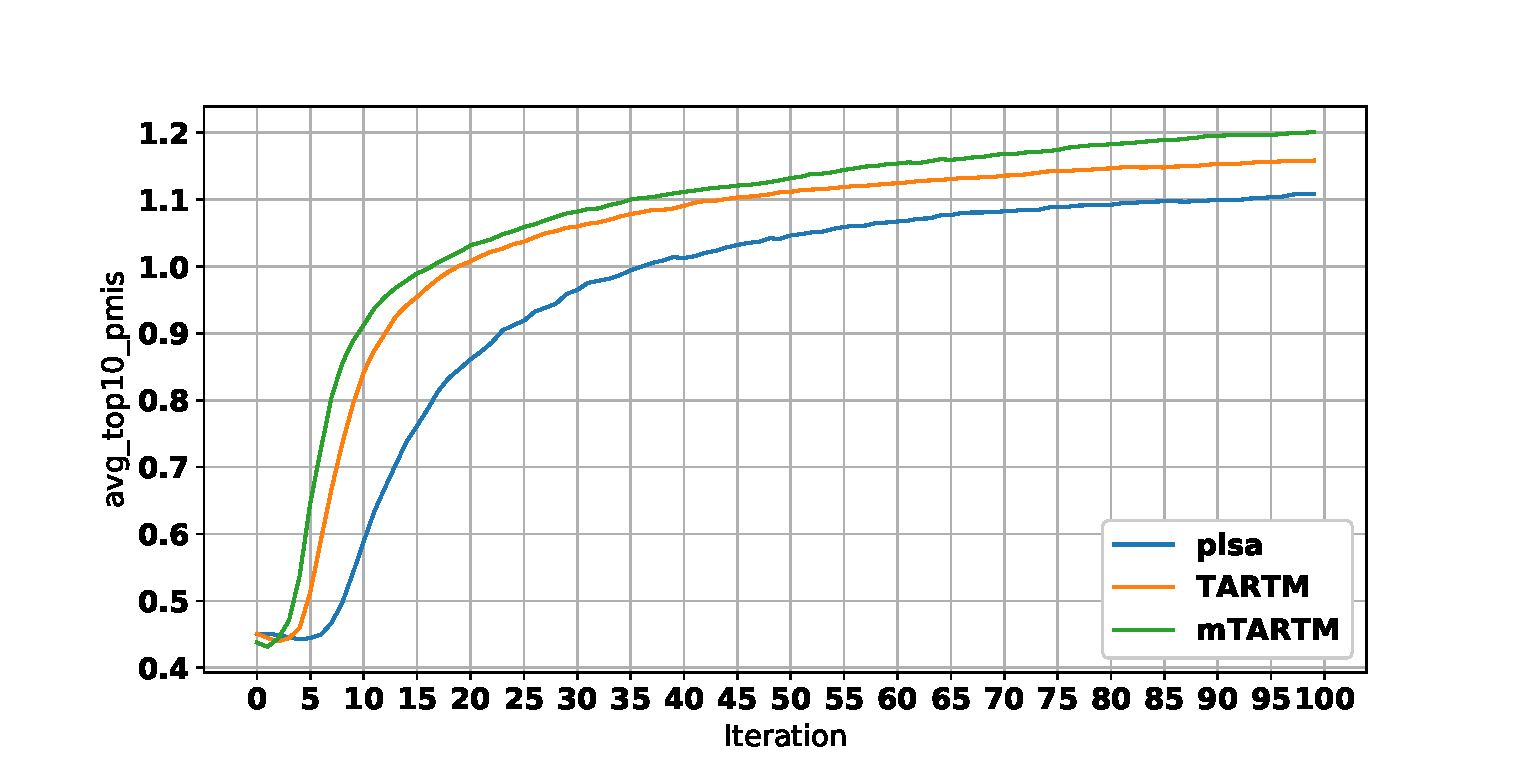
\includegraphics[width=.5\linewidth]{pictures/20news_10t_avg_top10_pmis.eps} &
    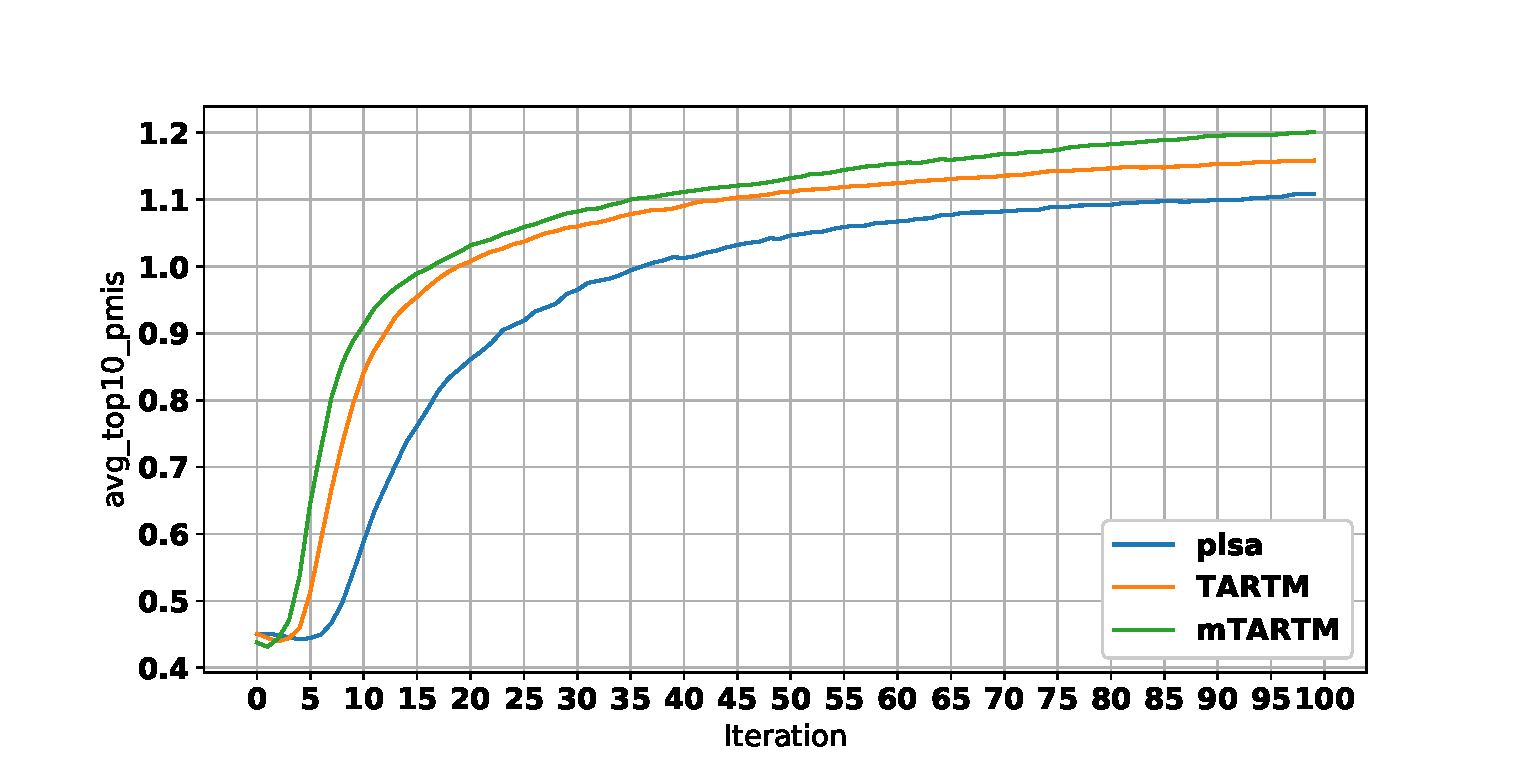
\includegraphics[width=.5\linewidth]{pictures/20news_10t_avg_top10_pmis.eps} 
  \end{tabular}
  \caption{20 news group, $|T| = 10$, pmi values}
\end{figure}

\begin{figure}[htb]
\centering
  \begin{tabular}{@{}cc@{}}
    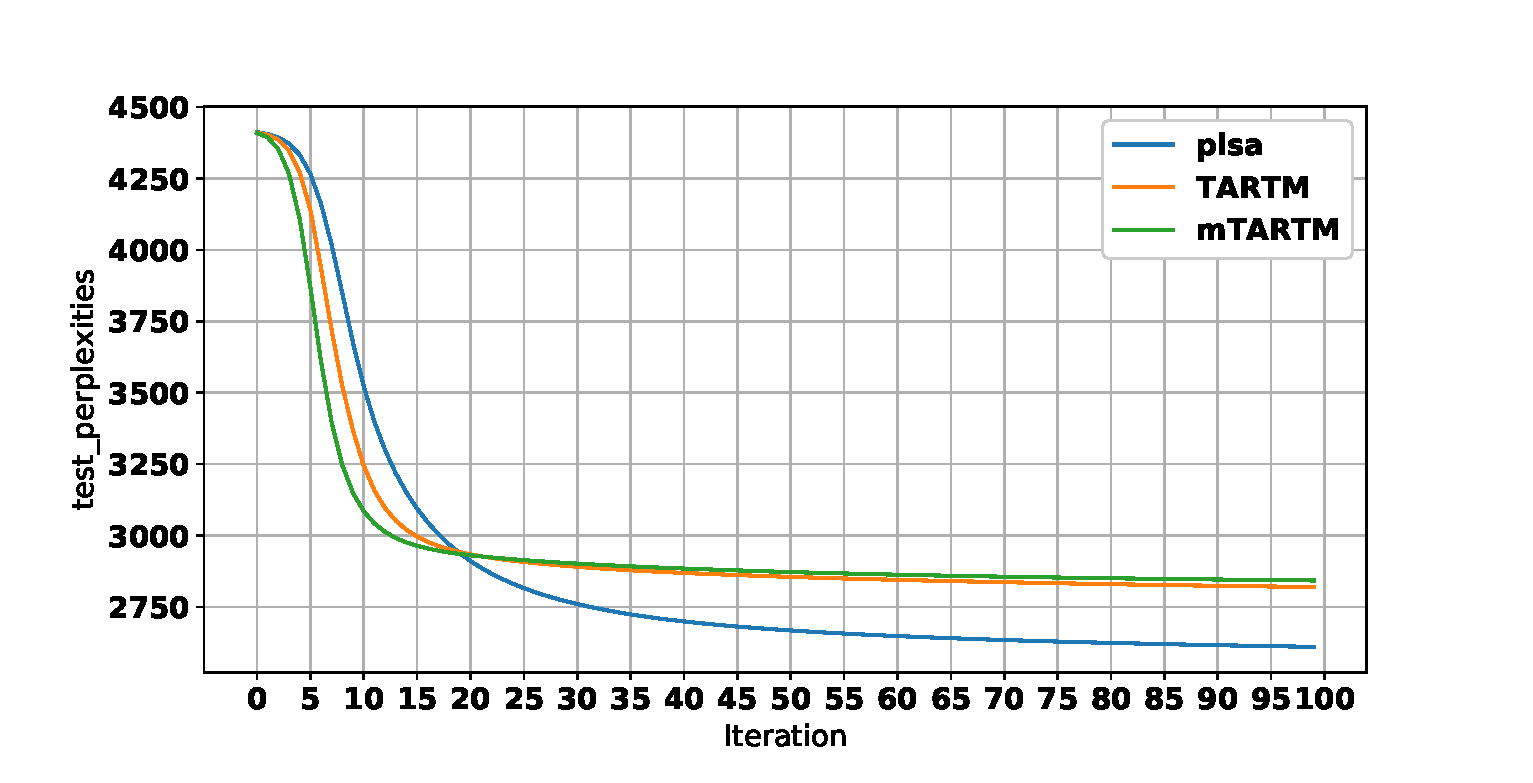
\includegraphics[width=.5\linewidth]{pictures/20news_10t_test_perplexities.eps} &
    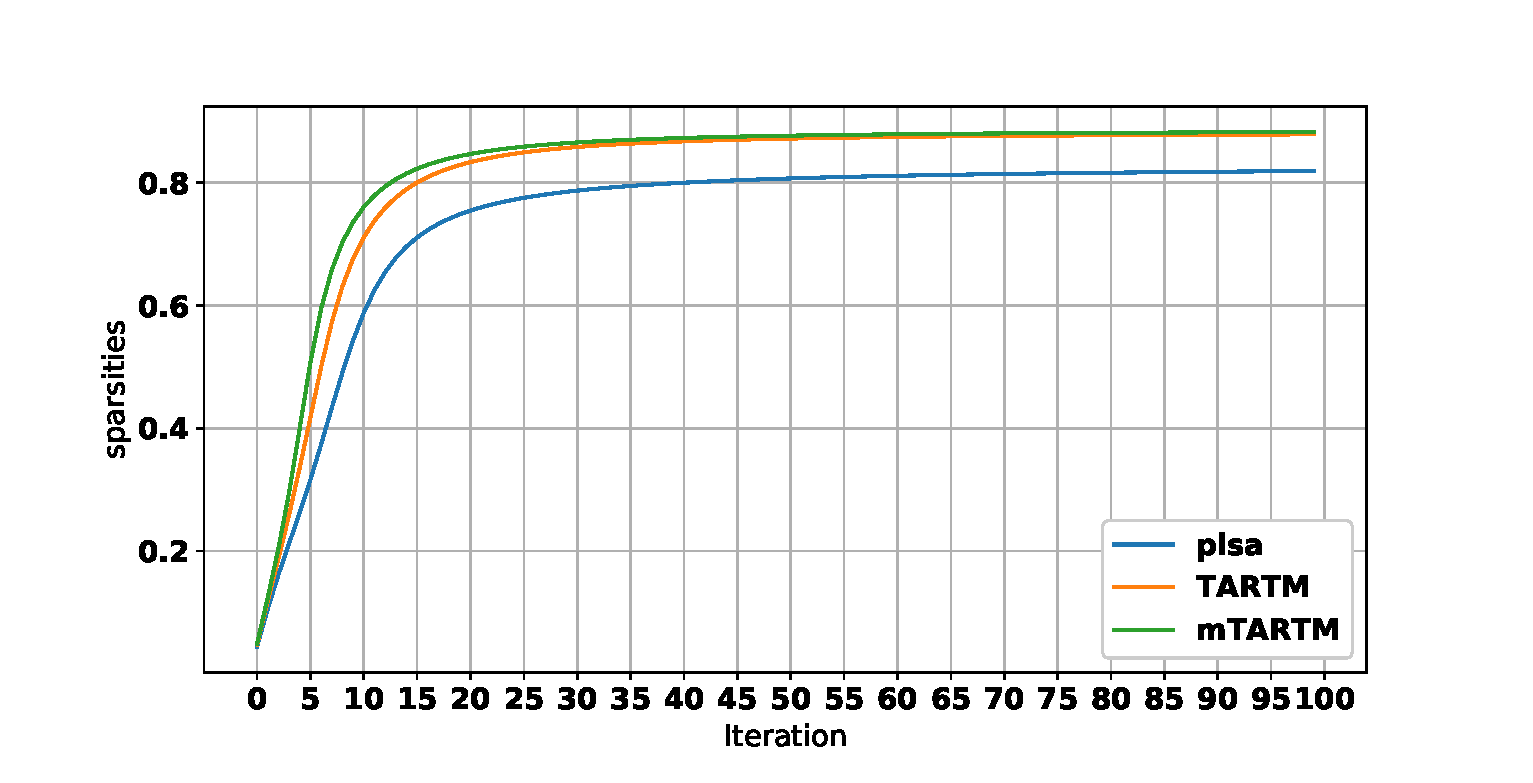
\includegraphics[width=.5\linewidth]{pictures/20news_10t_sparsities.eps} \\
    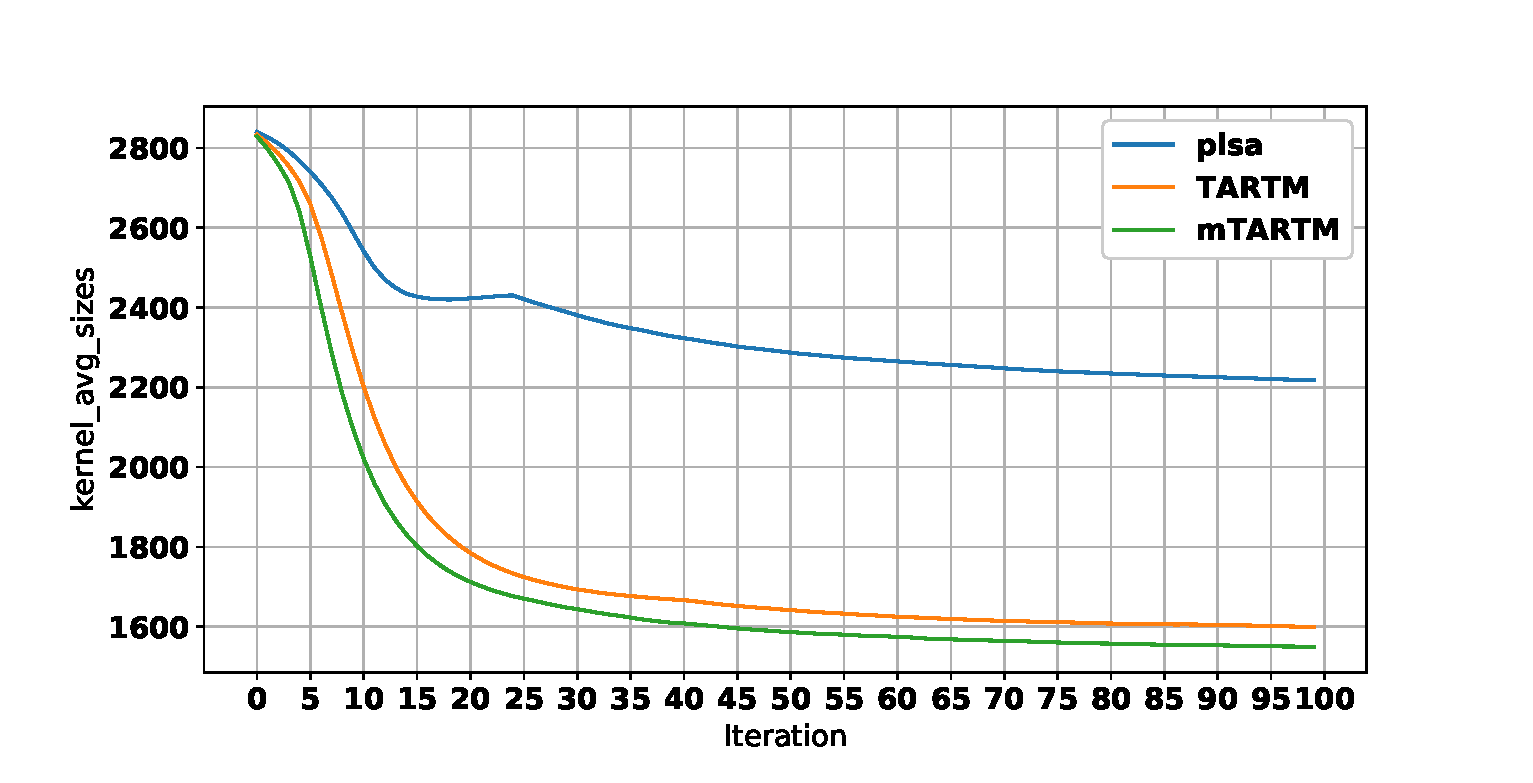
\includegraphics[width=.5\linewidth]{pictures/20news_10t_kernel_avg_sizes.eps} &
    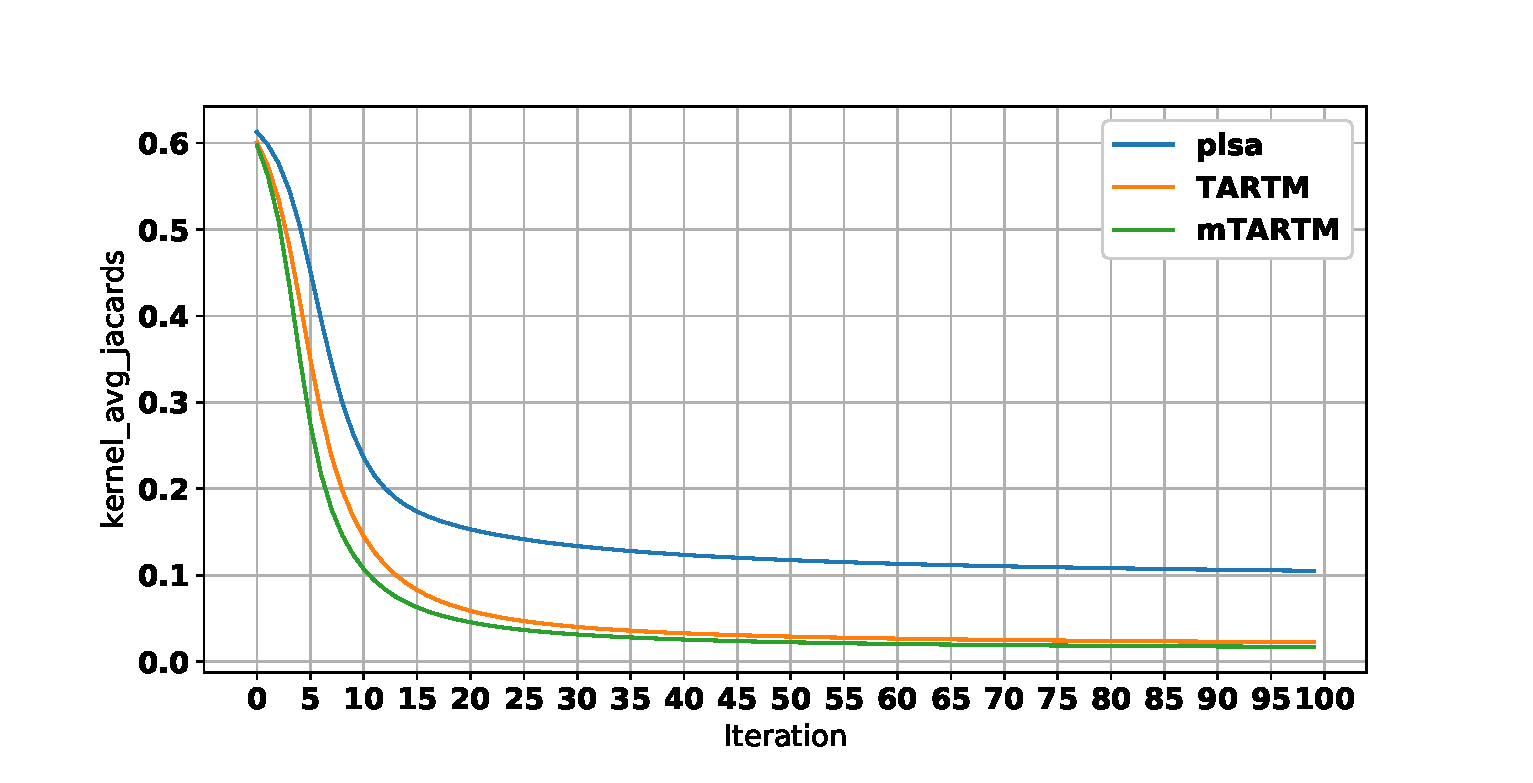
\includegraphics[width=.5\linewidth]{pictures/20news_10t_kernel_avg_jacards.eps} \\
  \end{tabular}
  \caption{20 news group, $|T| = 10$, other stats}
\end{figure}

\begin{figure}[htb]
\centering
  \begin{tabular}{@{}cc@{}}
    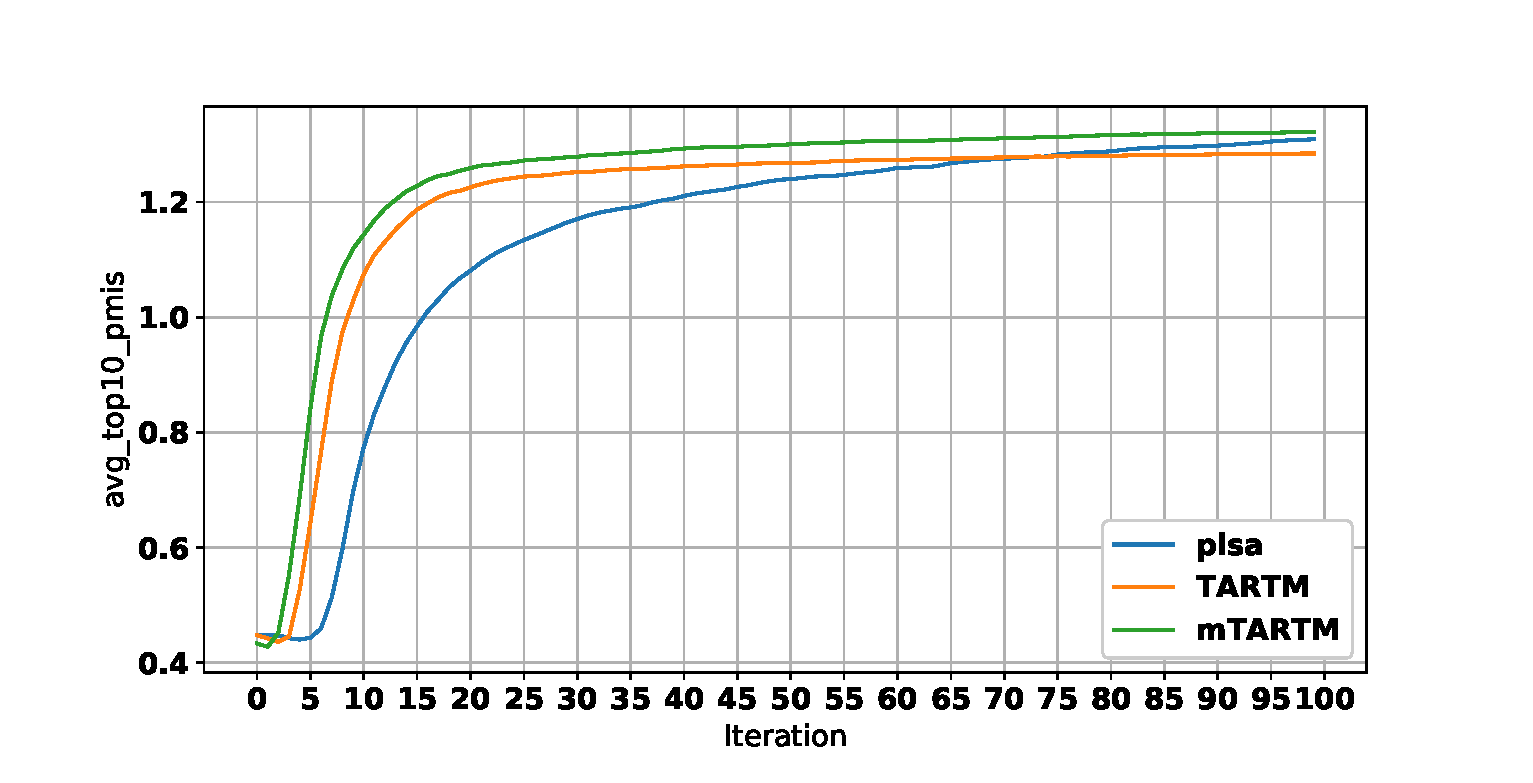
\includegraphics[width=.5\linewidth]{pictures/20news_25t_avg_top10_pmis.eps} &
    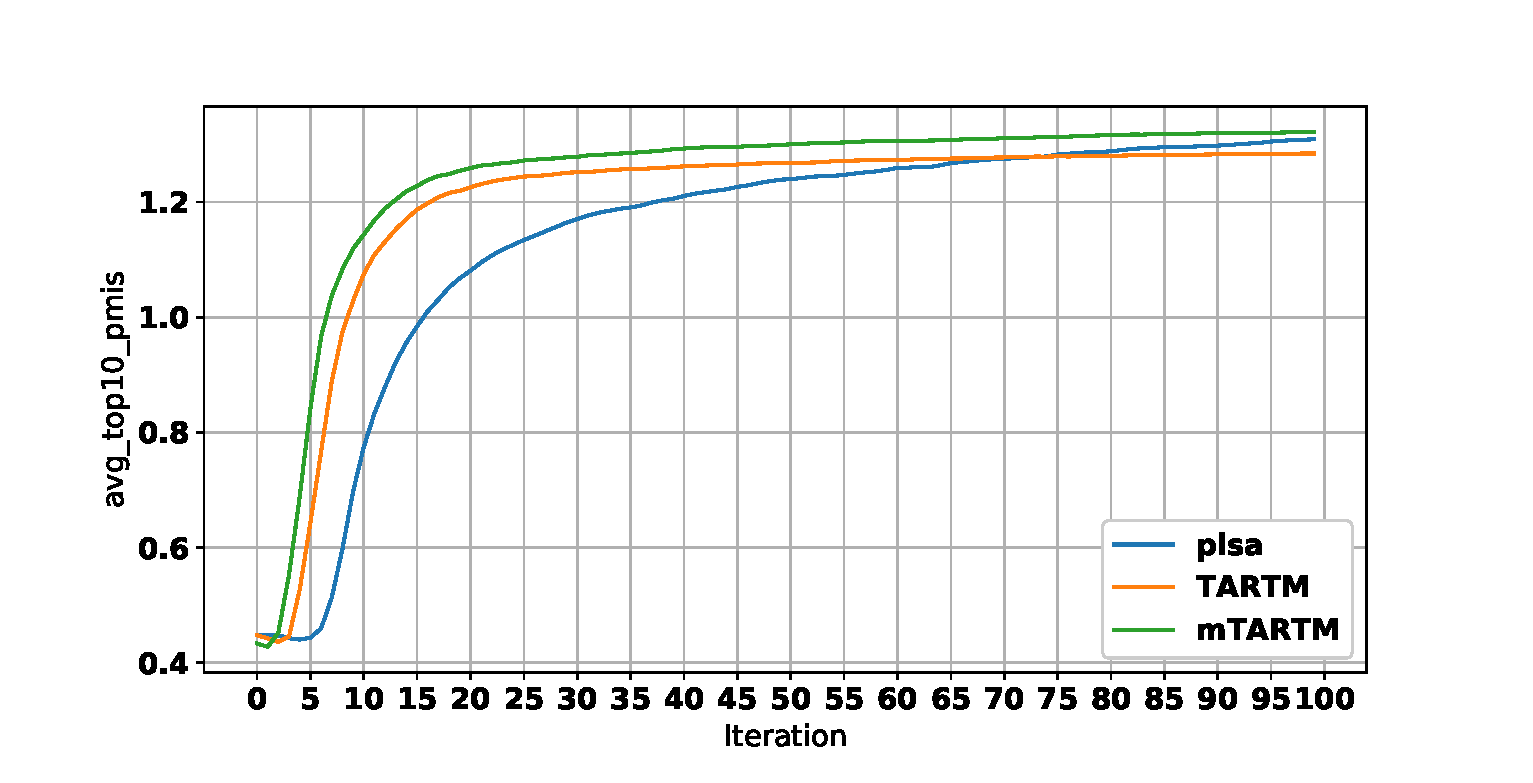
\includegraphics[width=.5\linewidth]{pictures/20news_25t_avg_top10_pmis.eps} 
  \end{tabular}
  \caption{20 news group, $|T| = 25$, pmi values}
\end{figure}

\begin{figure}[htb]
\centering
  \begin{tabular}{@{}cc@{}}
    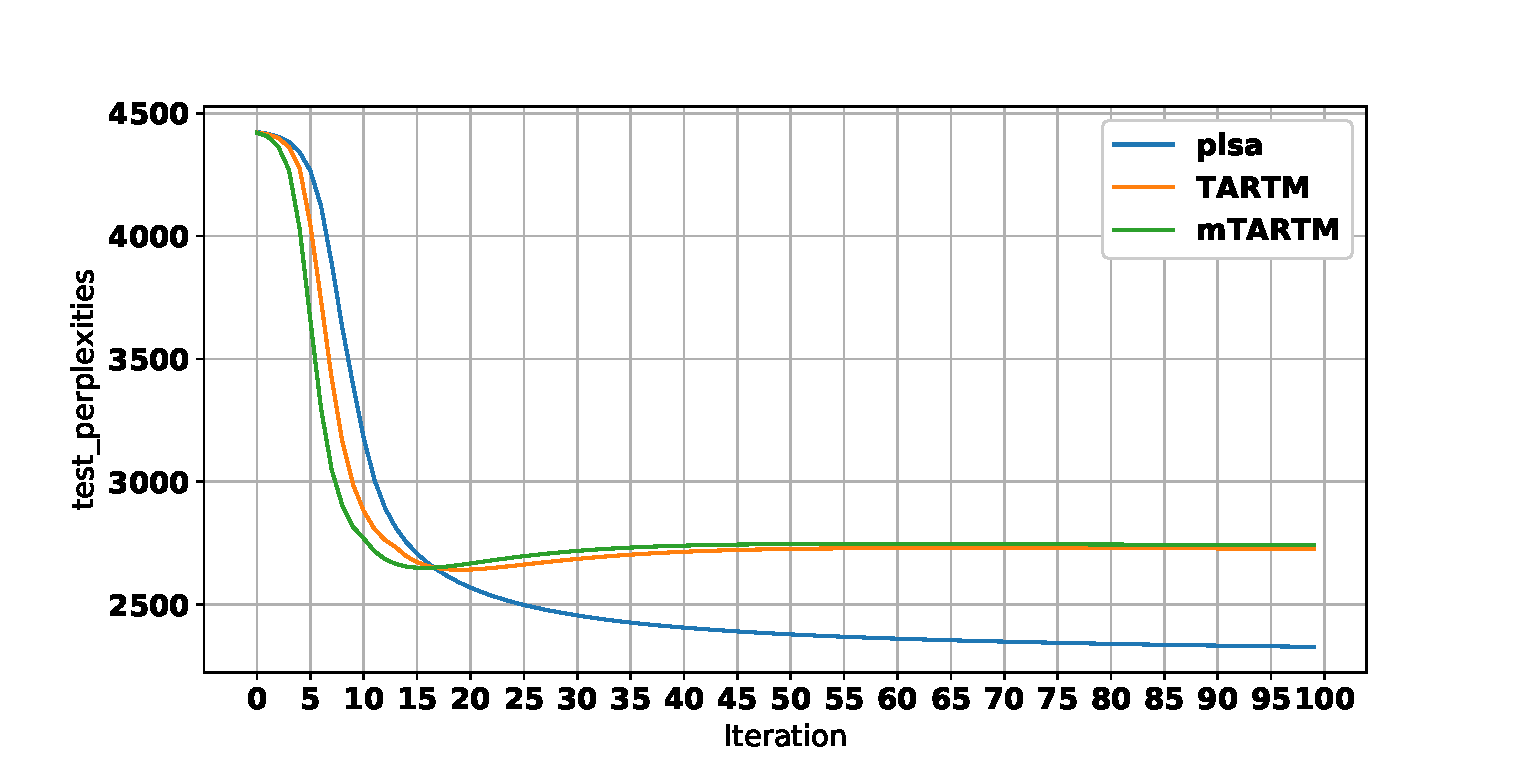
\includegraphics[width=.5\linewidth]{pictures/20news_25t_test_perplexities.eps} &
    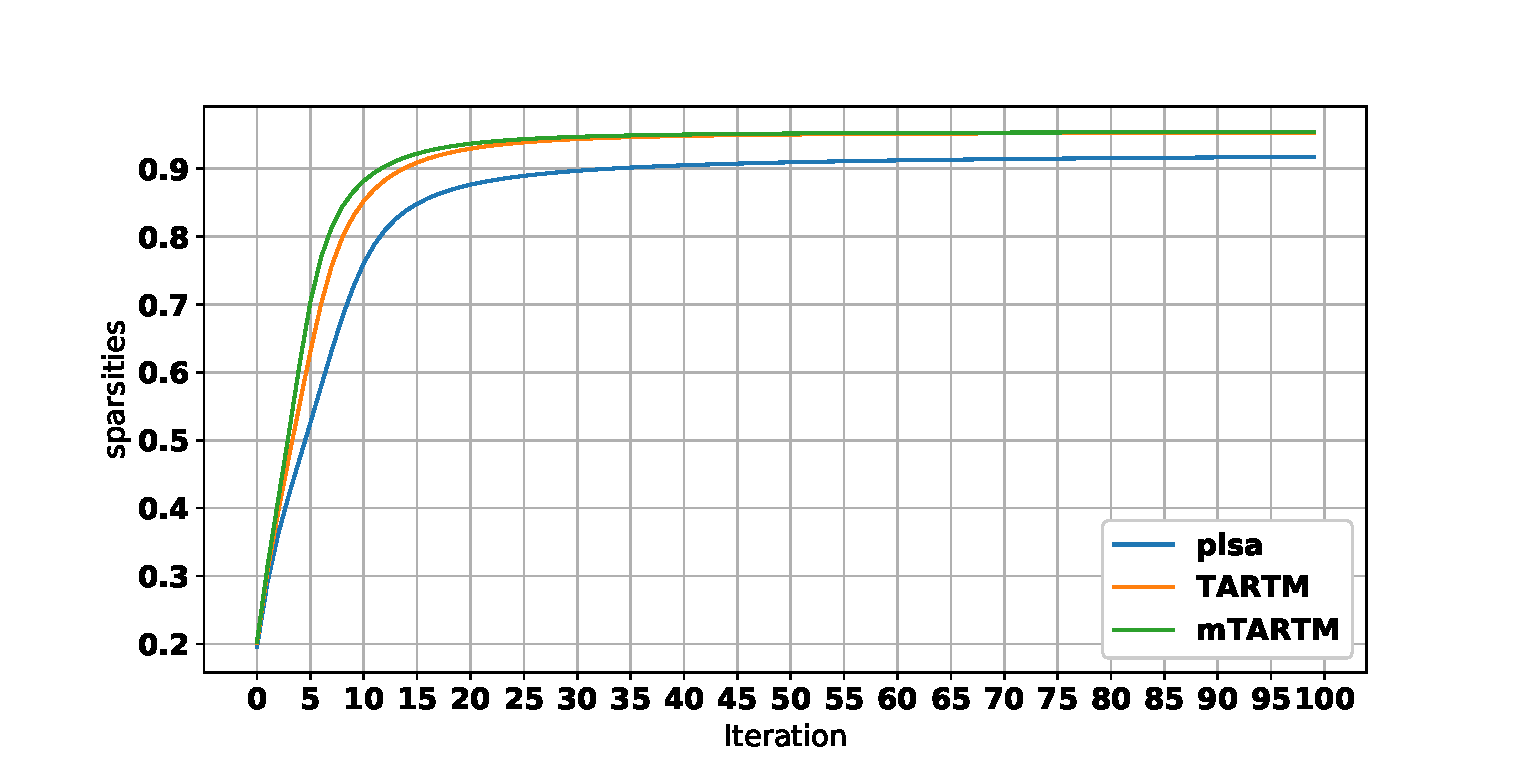
\includegraphics[width=.5\linewidth]{pictures/20news_25t_sparsities.eps} \\
    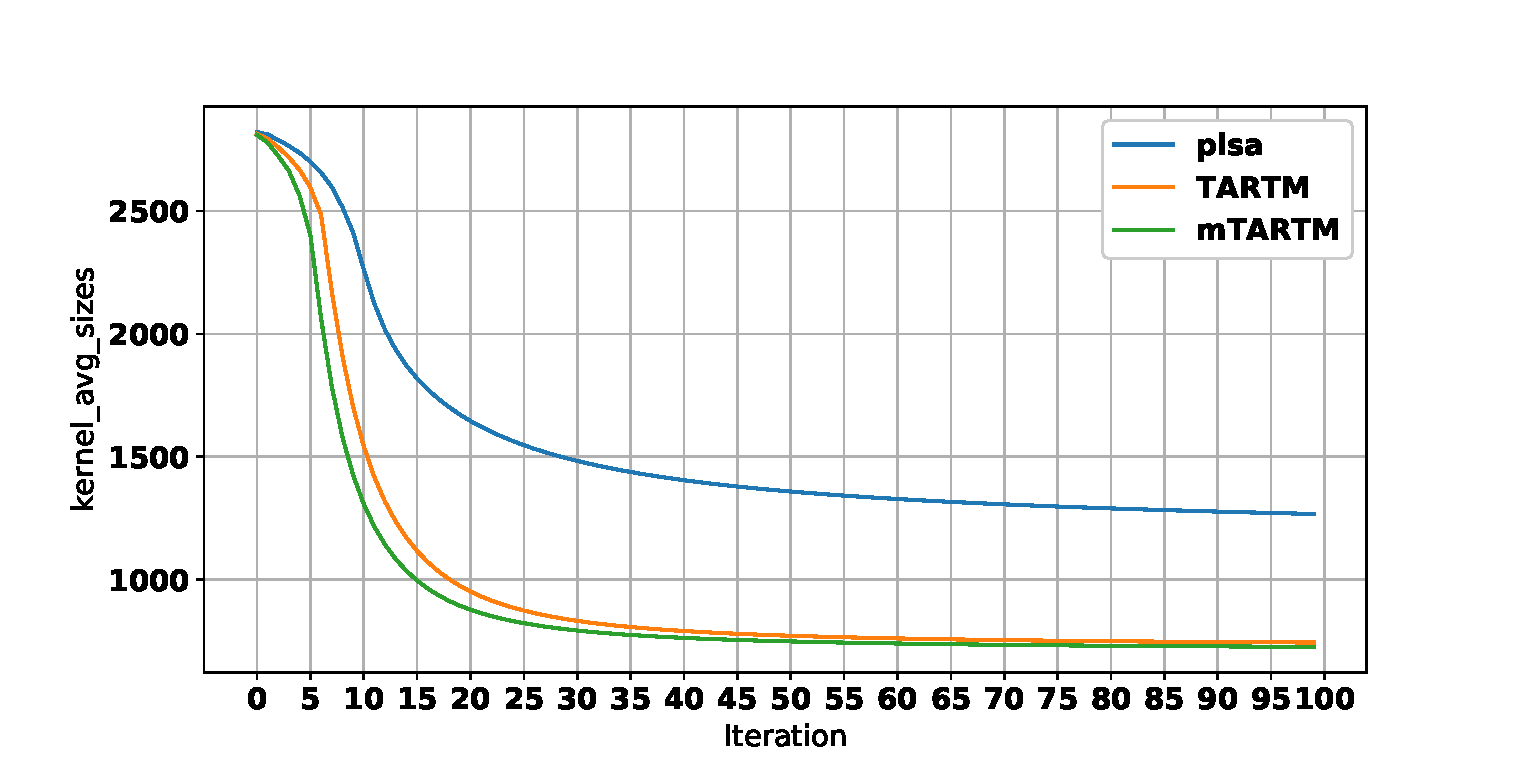
\includegraphics[width=.5\linewidth]{pictures/20news_25t_kernel_avg_sizes.eps} &
    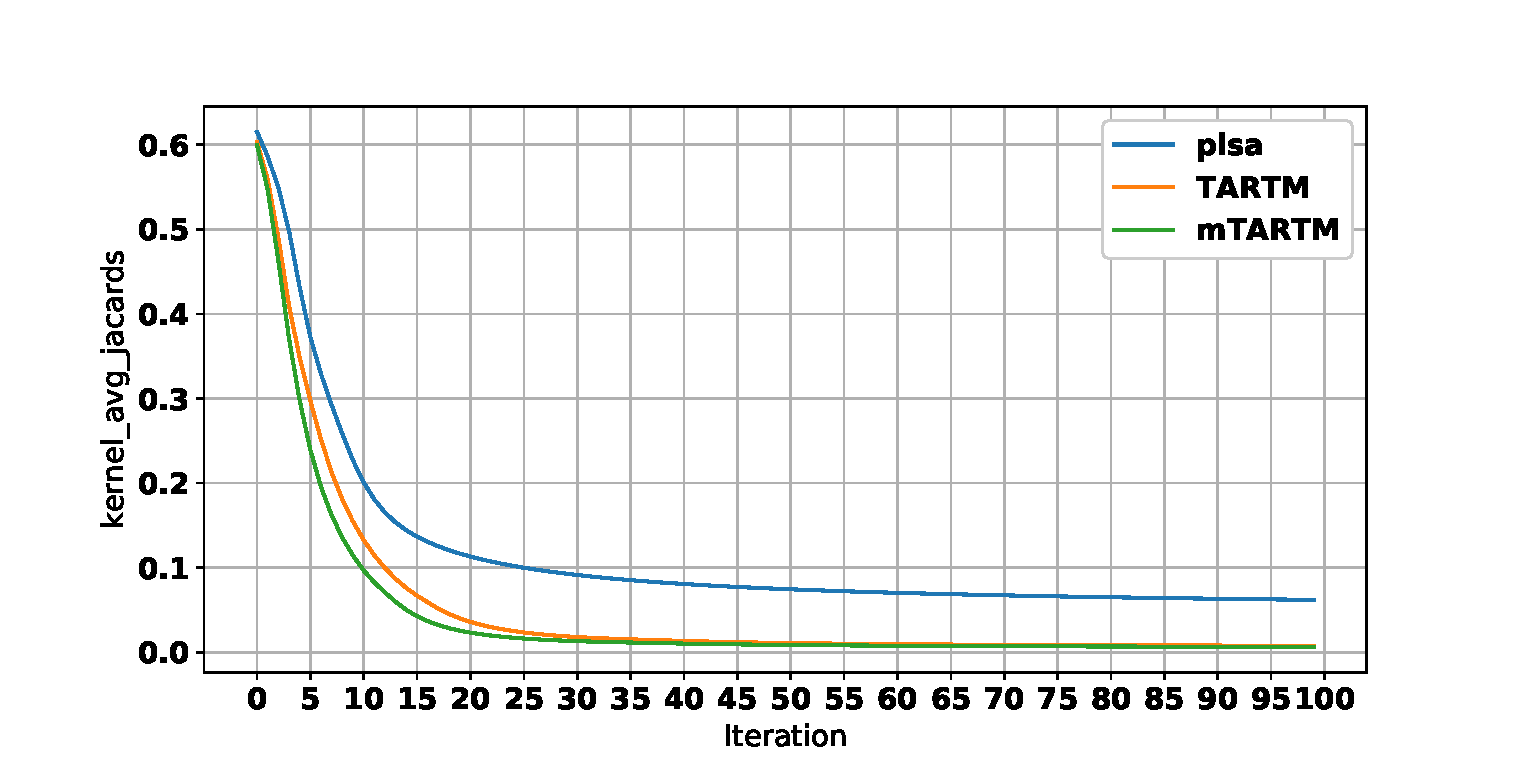
\includegraphics[width=.5\linewidth]{pictures/20news_25t_kernel_avg_jacards.eps} \\
  \end{tabular}
  \caption{20 news group, $|T| = 25$, other stats}
\end{figure}

\begin{figure}[htb]
\centering
  \begin{tabular}{@{}cc@{}}
    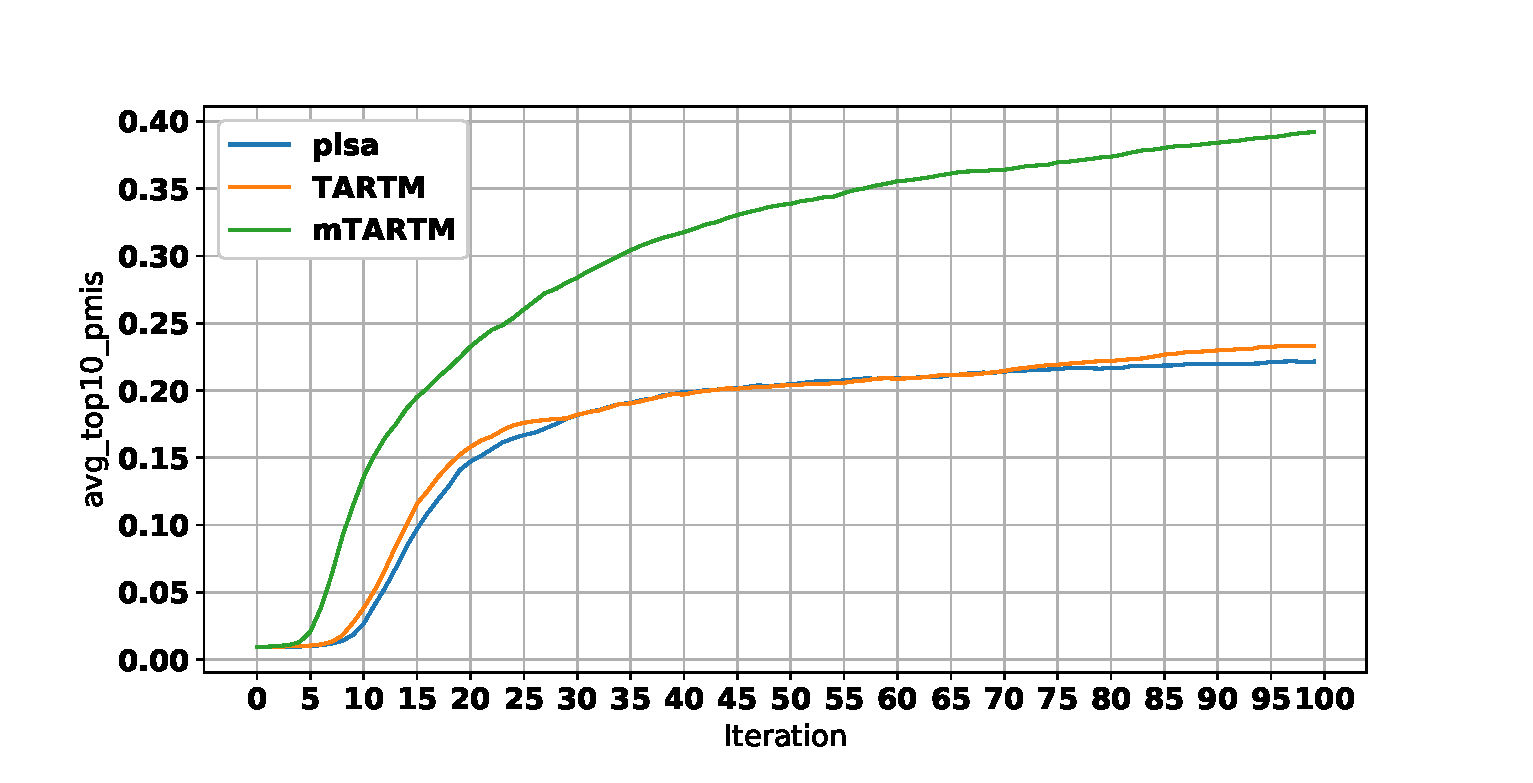
\includegraphics[width=.5\linewidth]{pictures/NIPS_20t_avg_top10_pmis.eps} &
    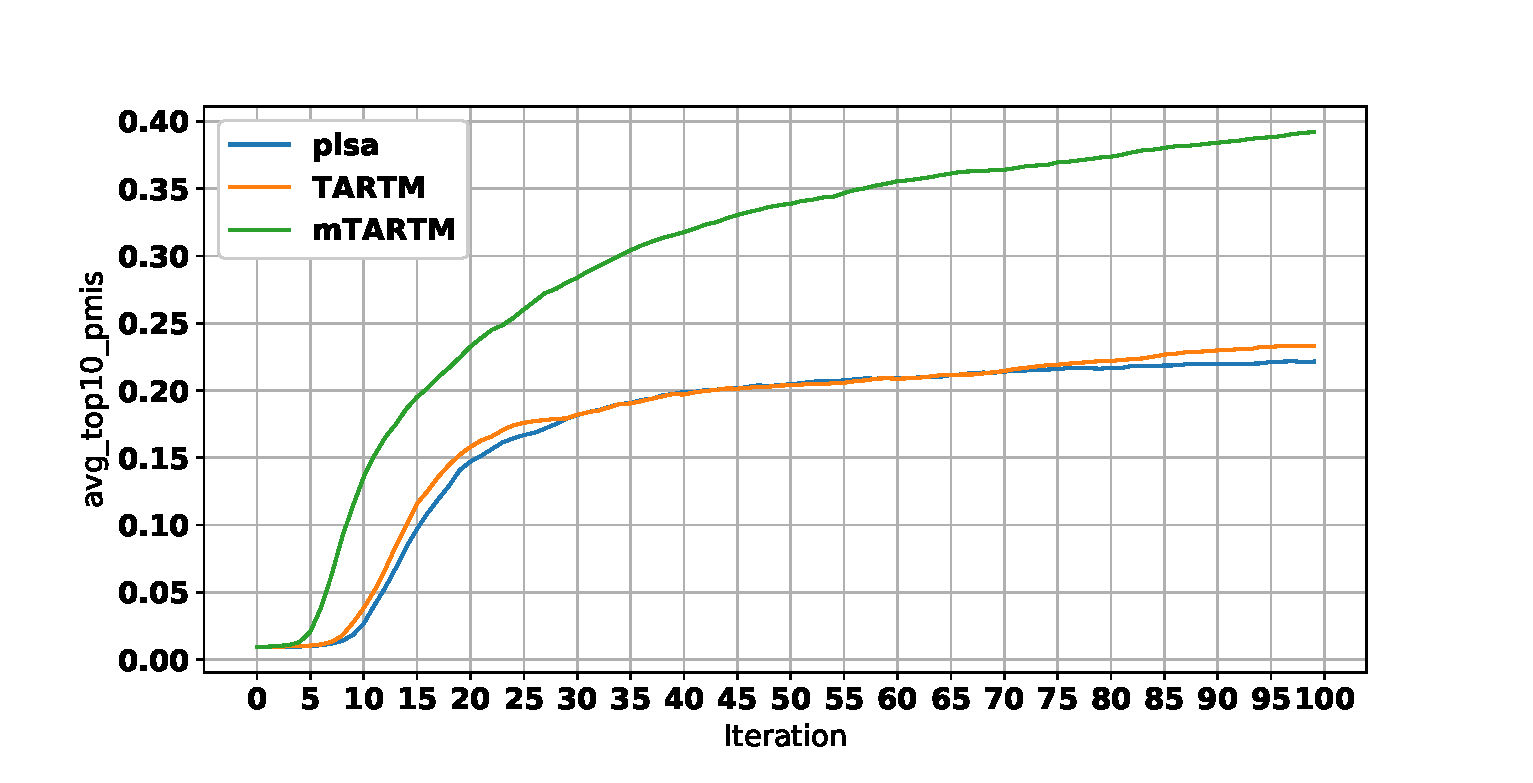
\includegraphics[width=.5\linewidth]{pictures/NIPS_20t_avg_top10_pmis.eps} 
  \end{tabular}
  \caption{NIPS, $|T| = 20$, pmi values}
\end{figure}

\begin{figure}[htb]
\centering
  \begin{tabular}{@{}cc@{}}
    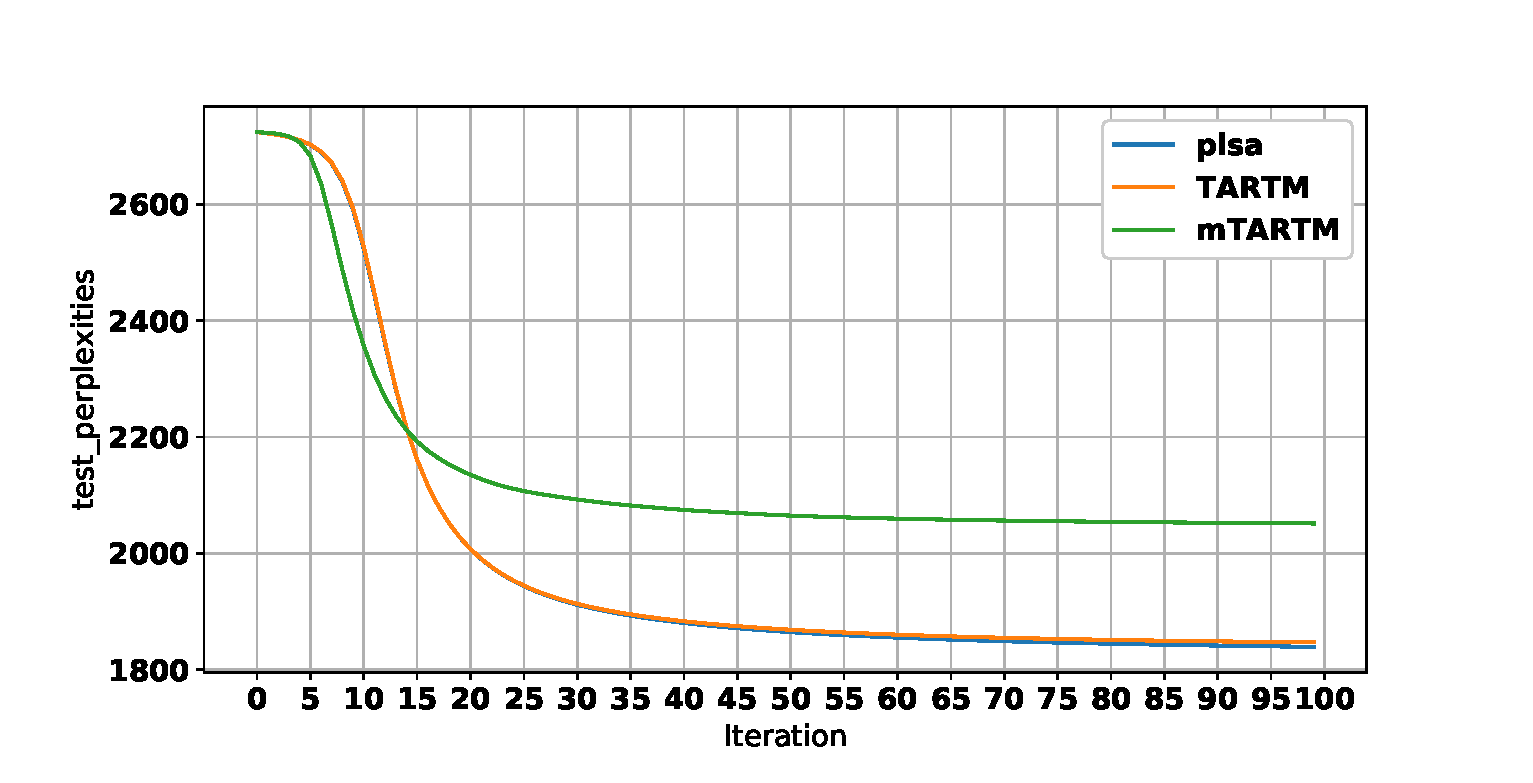
\includegraphics[width=.5\linewidth]{pictures/NIPS_20t_test_perplexities.eps} &
    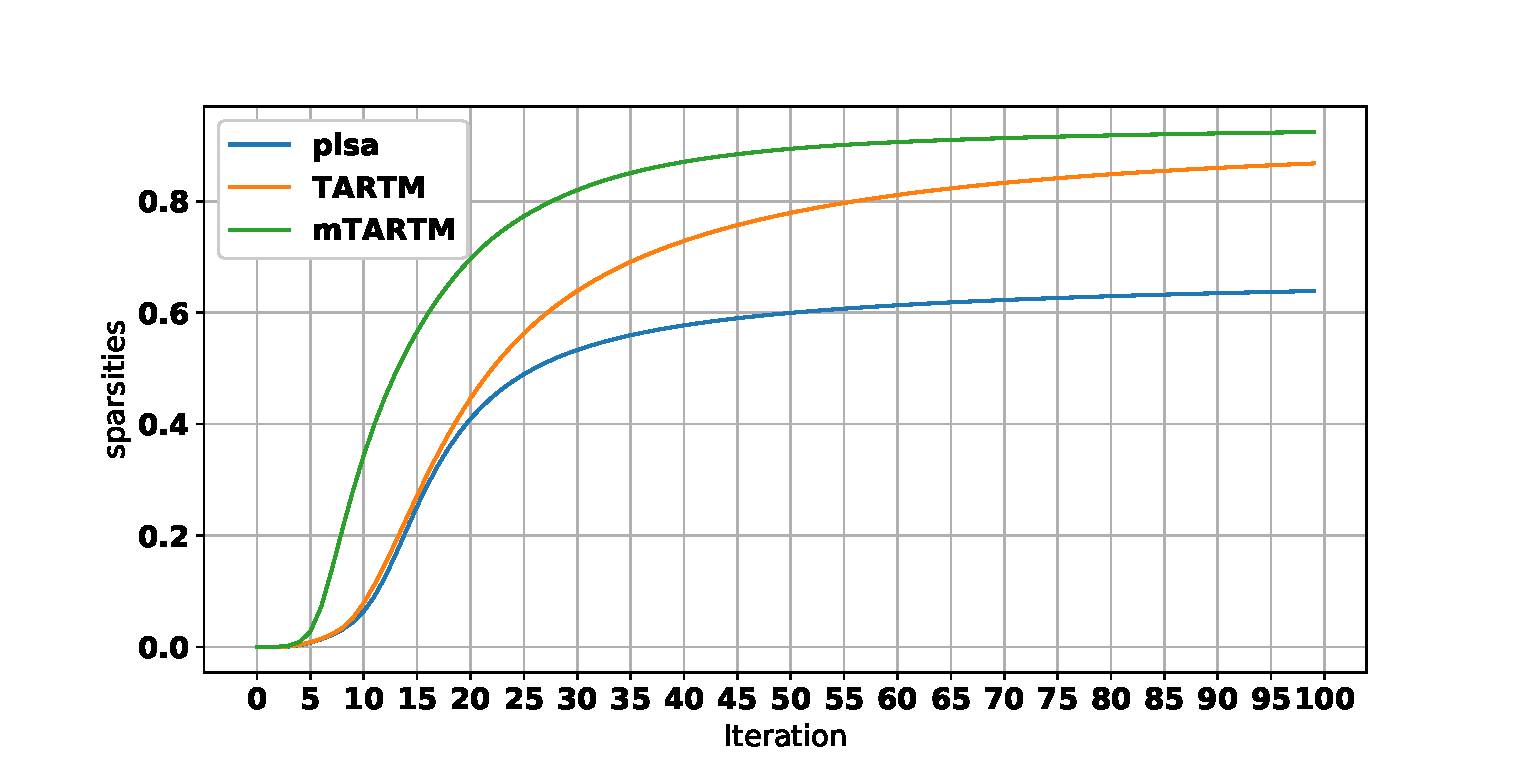
\includegraphics[width=.5\linewidth]{pictures/NIPS_20t_sparsities.eps} \\
    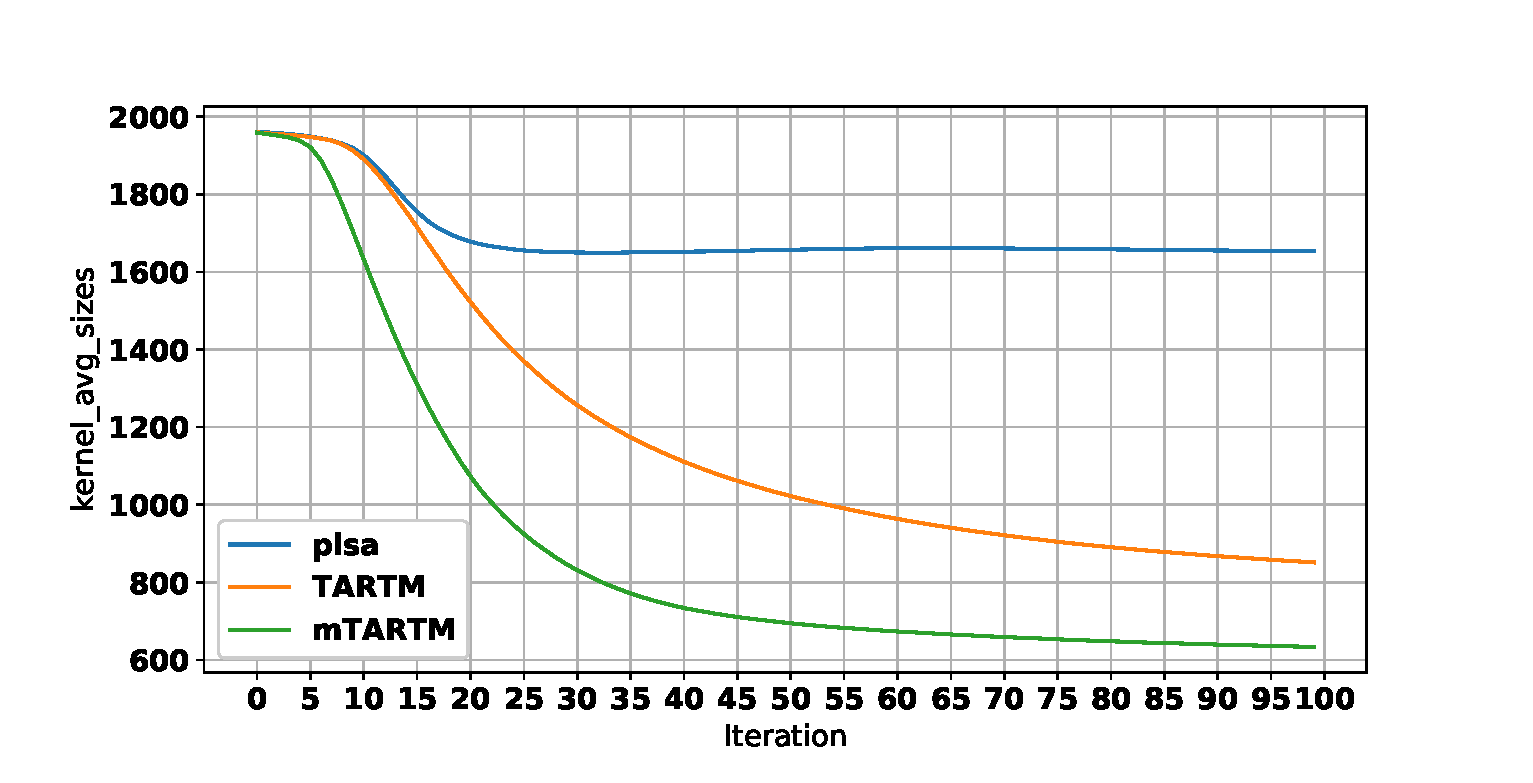
\includegraphics[width=.5\linewidth]{pictures/NIPS_20t_kernel_avg_sizes.eps} &
    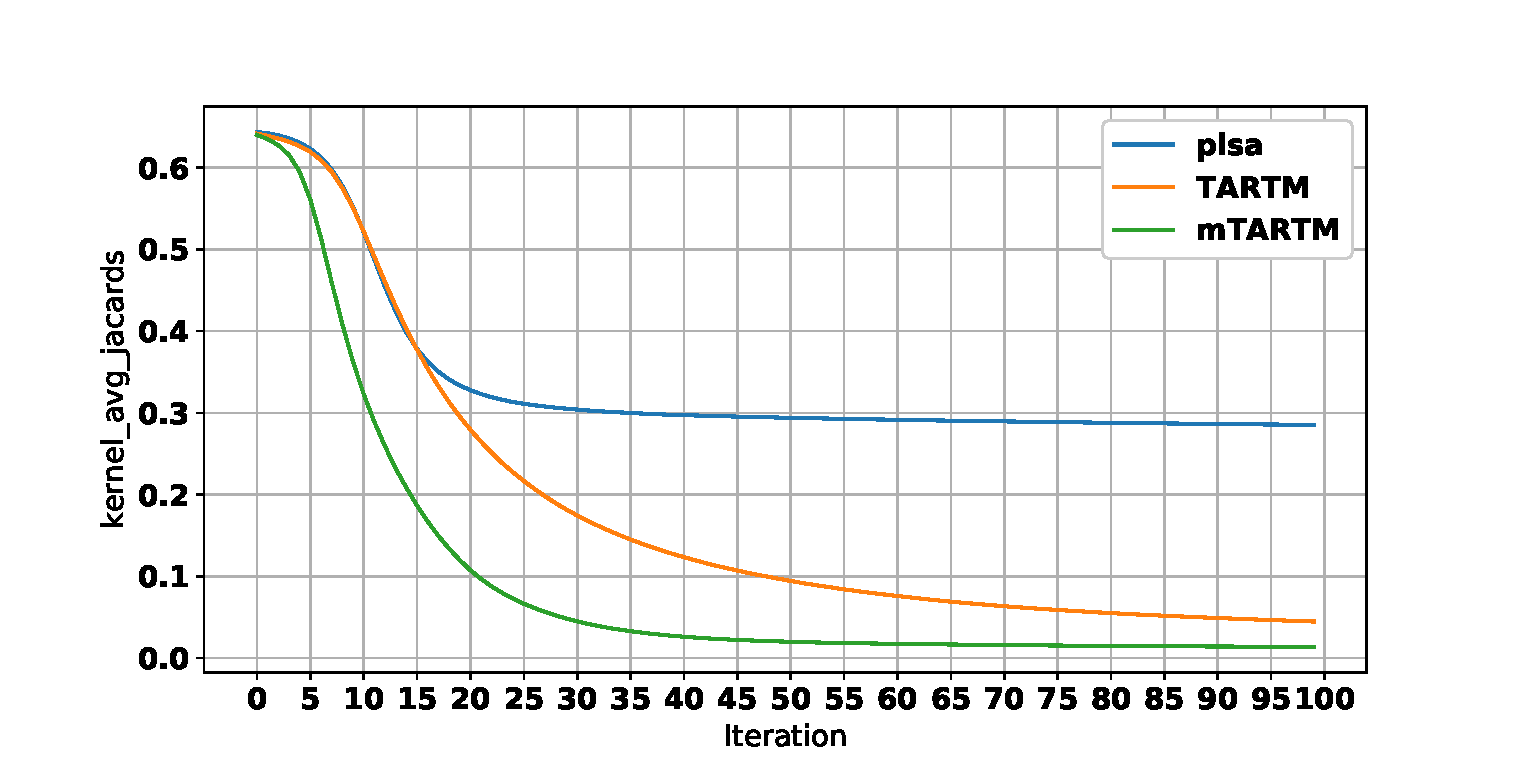
\includegraphics[width=.5\linewidth]{pictures/NIPS_20t_kernel_avg_jacards.eps} \\
  \end{tabular}
  \caption{NIPS, $|T| = 20$, other stats}
\end{figure}

\begin{figure}[htb]
\centering
  \begin{tabular}{@{}cc@{}}
    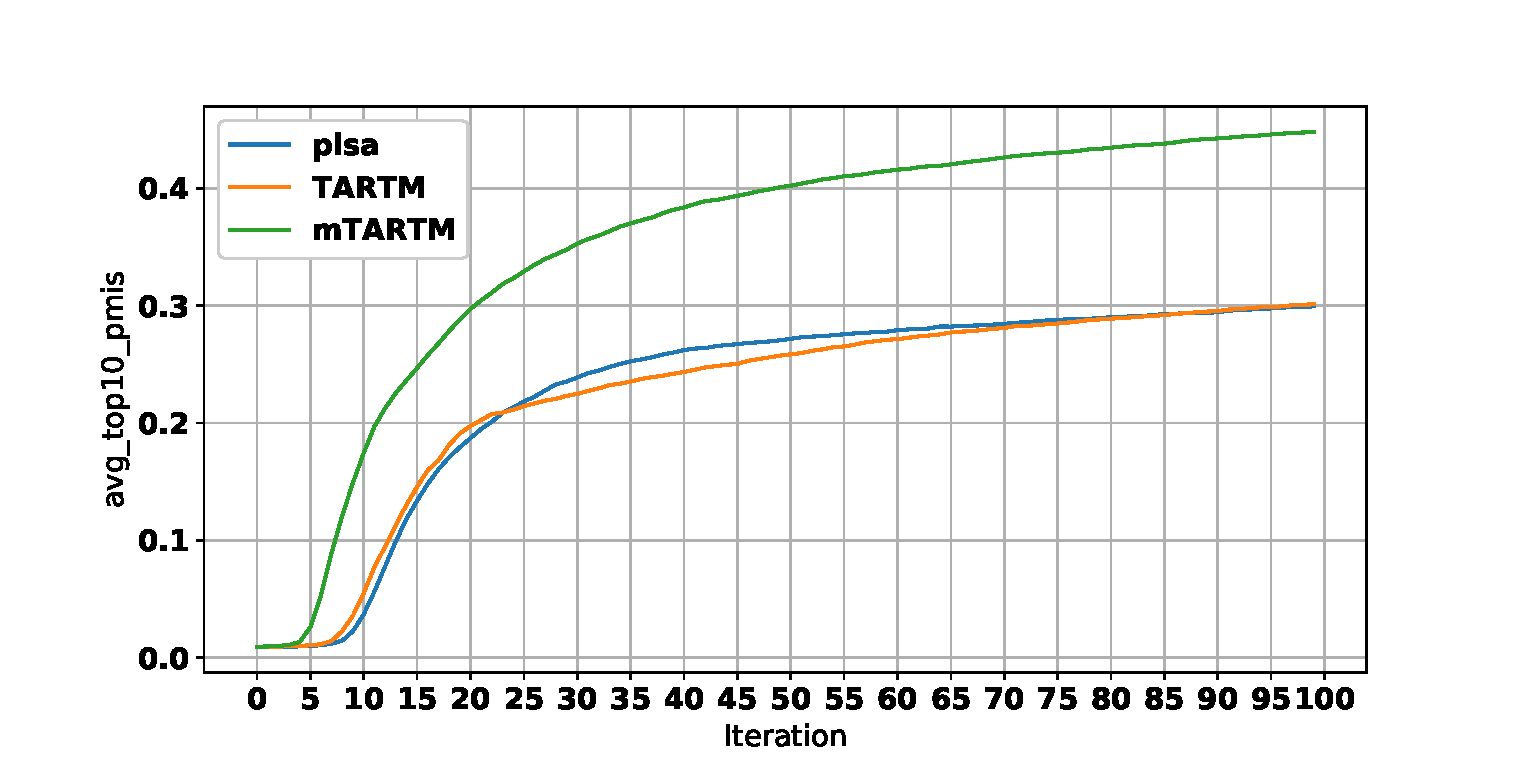
\includegraphics[width=.5\linewidth]{pictures/NIPS_50t_avg_top10_pmis.eps} &
    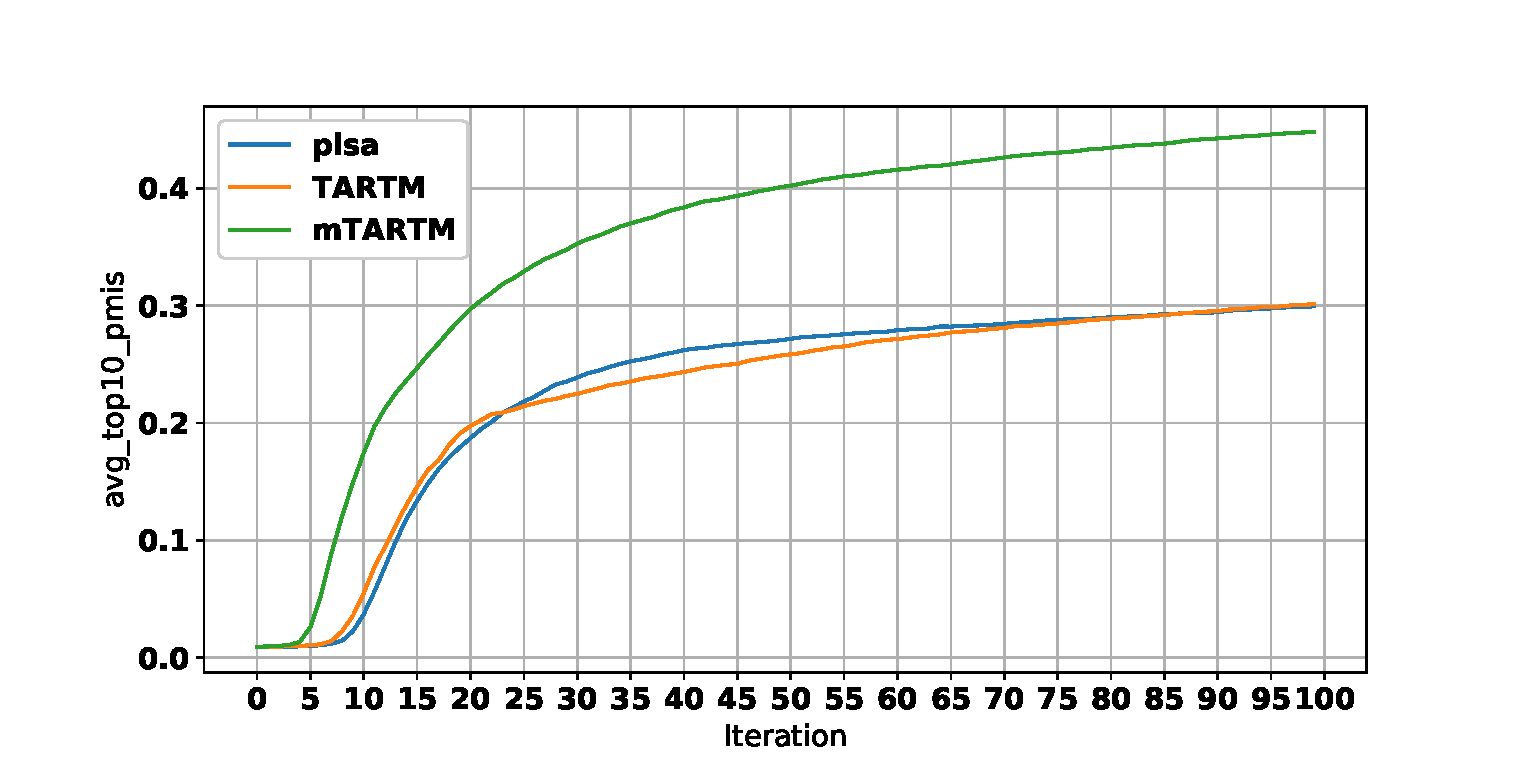
\includegraphics[width=.5\linewidth]{pictures/NIPS_50t_avg_top10_pmis.eps} 
  \end{tabular}
  \caption{NIPS, $|T| = 50$, pmi values}
\end{figure}

\begin{figure}[htb]
\centering
  \begin{tabular}{@{}cc@{}}
    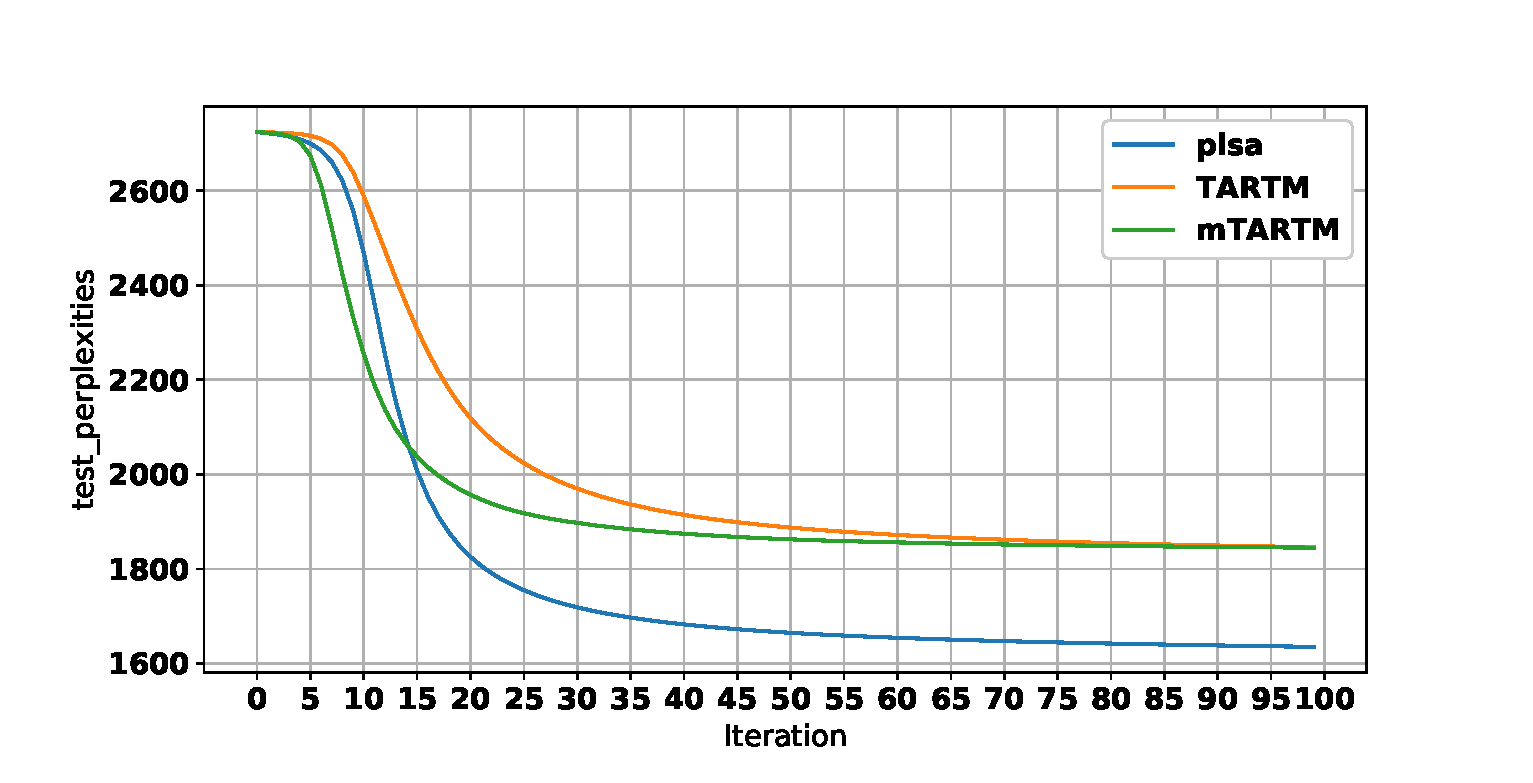
\includegraphics[width=.5\linewidth]{pictures/NIPS_50t_test_perplexities.eps} &
    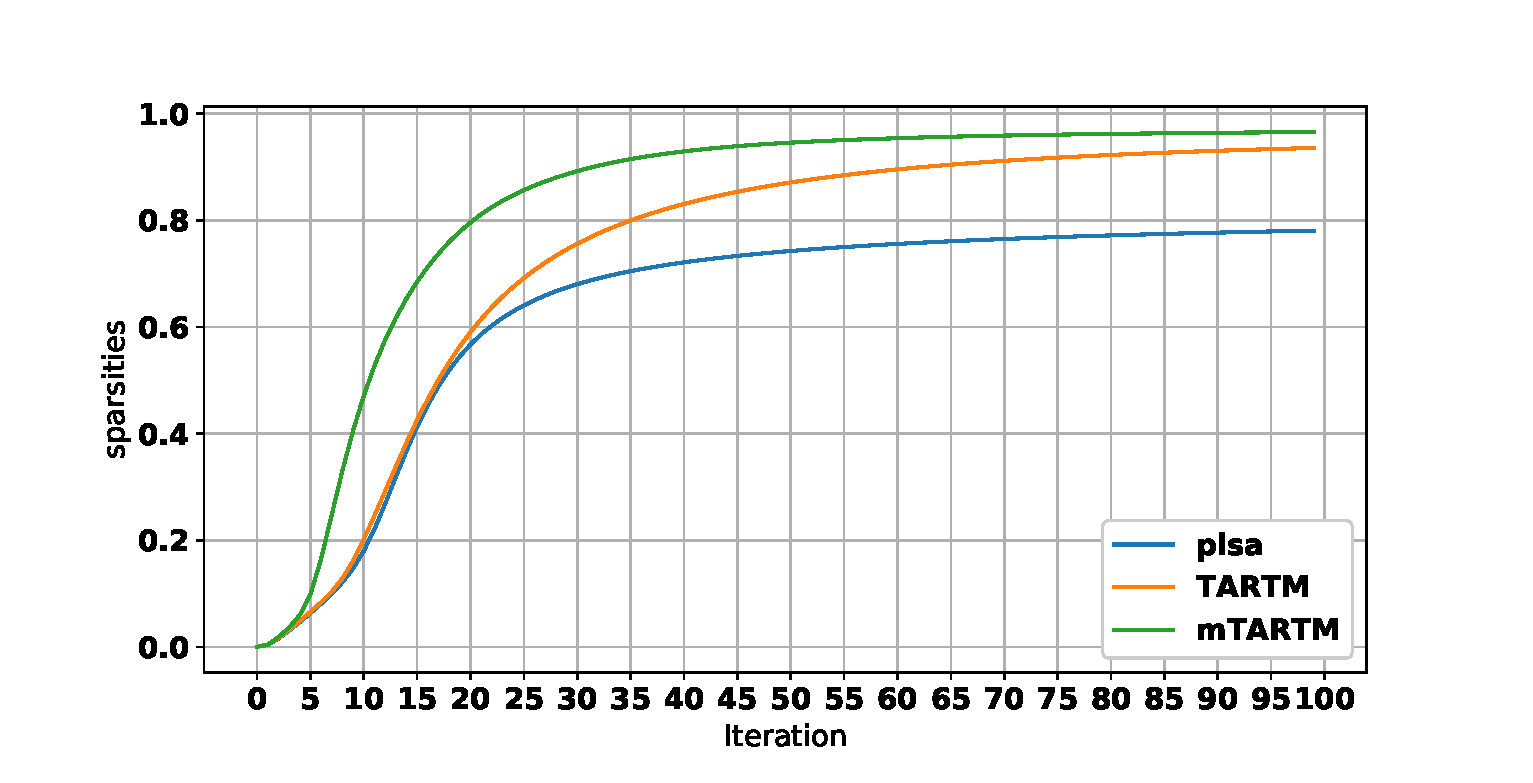
\includegraphics[width=.5\linewidth]{pictures/NIPS_50t_sparsities.eps} \\
    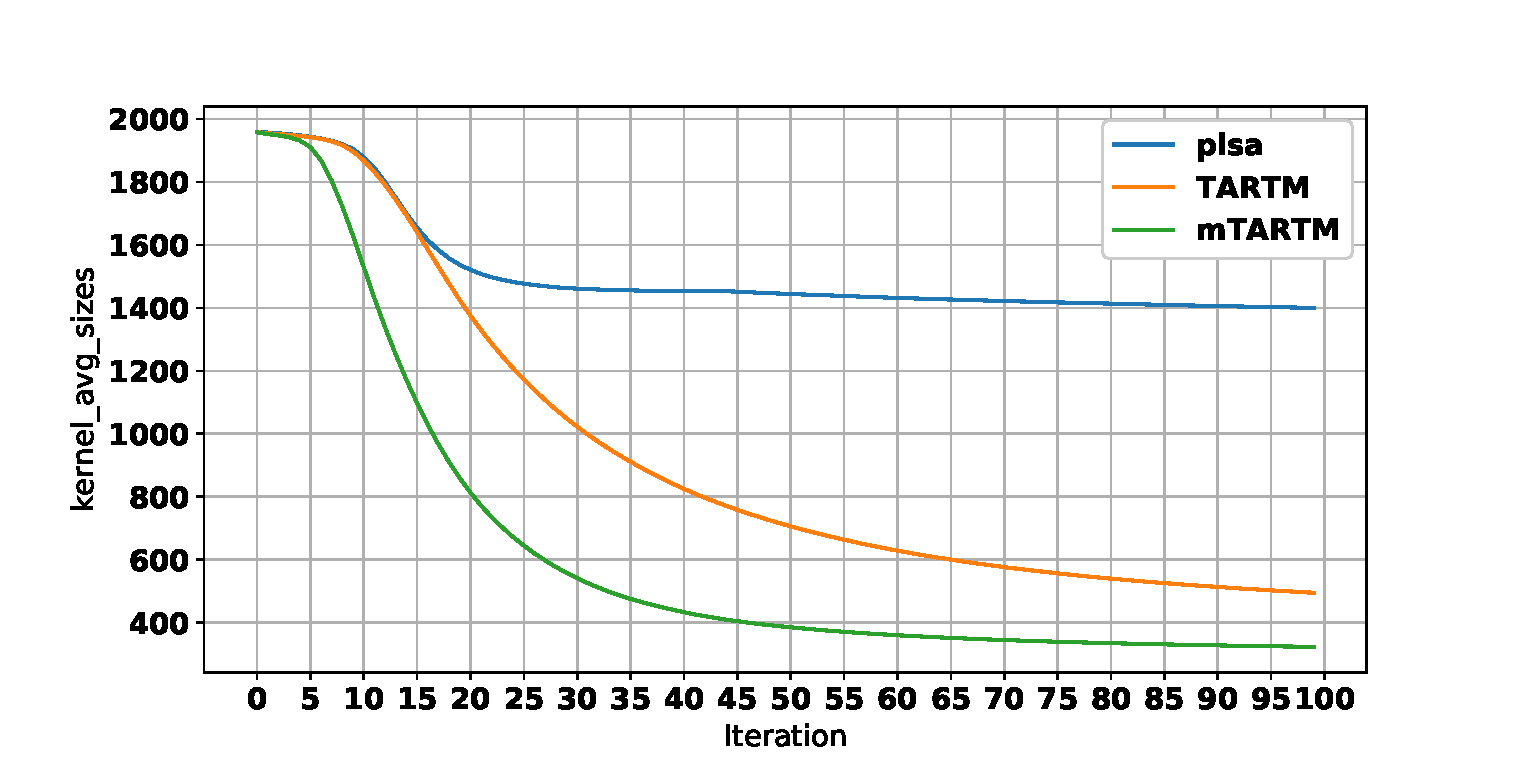
\includegraphics[width=.5\linewidth]{pictures/NIPS_50t_kernel_avg_sizes.eps} &
    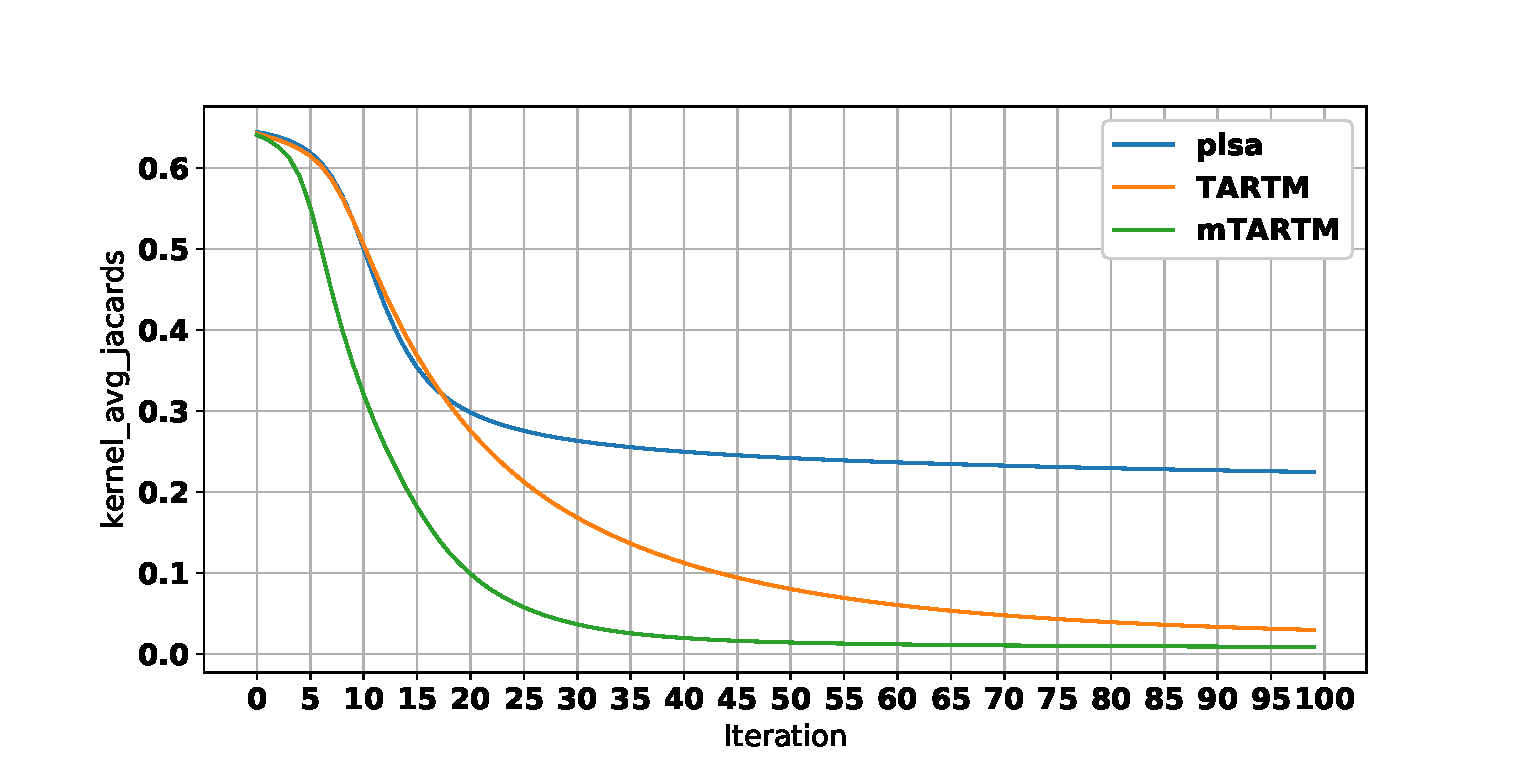
\includegraphics[width=.5\linewidth]{pictures/NIPS_50t_kernel_avg_jacards.eps} \\
  \end{tabular}
  \caption{NIPS, $|T| = 50$, other stats}
\end{figure}

\end{document}